\documentclass[hidelinks,12pt]{article}
\usepackage[a4paper,width=150mm,top=25mm,bottom=25mm]{geometry}
\usepackage[utf8]{inputenc}
\usepackage{graphicx}
\usepackage{lipsum}
\usepackage{amssymb}
\usepackage{apacite}
\usepackage{natbib}
\usepackage{hyperref}
\usepackage{float}
\usepackage{ragged2e}
\usepackage[font={footnotesize,bf}]{caption}
\usepackage[nottoc,numbib]{tocbibind}
\usepackage{multirow}
\usepackage{placeins}
\usepackage{booktabs}
\usepackage{hyperref}
\hypersetup{
    colorlinks=true,
    linkcolor=blue,
    filecolor=magenta,      
    urlcolor=cyan,
    pdftitle={Overleaf Example},
    pdfpagemode=FullScreen,
    }
\renewcommand{\thesubsection}{\thesection.\alph{subsection}}

\linespread{1.5}

\begin{document}

\begin{titlepage}
    \begin{center}
        \vspace*{1cm}
        
        
        % \vfill
        
        \large
        \textbf{Big Data Asset Pricing \\ Exercise 4: Hig-Dimensional Return Predictions}
            
        
        \normalsize
        Seyyed Morteza Aghajanzadeh \\
        Department of Finance \\
        Stockholm School of Economics
        
        \vfill
        \normalsize
        \justifying
        \noindent
        \textbf{Statement:} I certify with my signature that I have solved the exercise according to the Code of Professional Conduct and Ethics. 
        For example, I have not plagiarized others, but, instead, solved the exercise myself (possibly with allowed collaboration with other students), and I have referenced my sources appropriately.

        \vfill
        
        \vspace{0.8cm}
            
        
        \vspace{0.8cm}
        \normalsize
        \centering
        2024-01
            
    \end{center}
\end{titlepage}

% Question 1
\section{}
\begin{figure}[htbp]
    \centering
    \caption{The number of stocks per month.}
    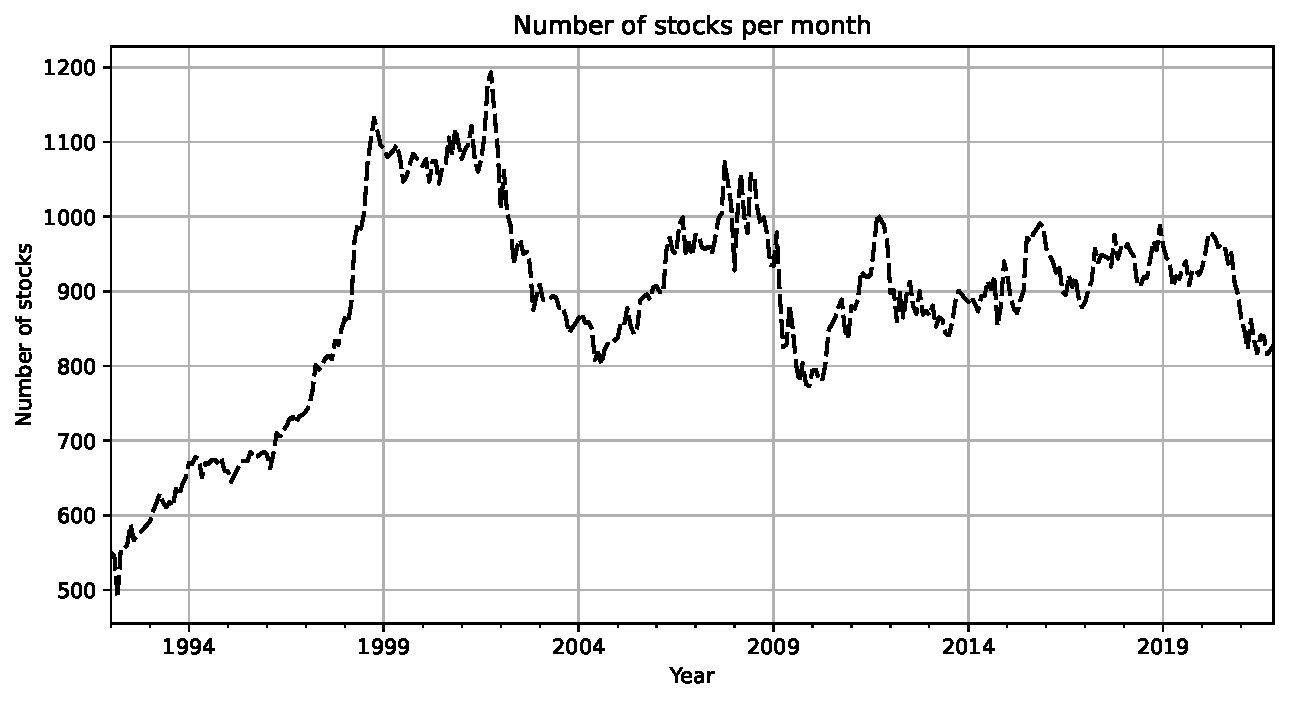
\includegraphics[width=.95\textwidth]{out/1.pdf}
\end{figure}

\FloatBarrier

% Question 2
\section{}
\subsection{}
\begin{table}[htbp]
    \centering
    \caption{The results of the Pooled OLS regression over training}
    \resizebox{.9\textwidth}{!}{\begin{tabular}{lcccccc}
\toprule
                        & \textbf{Parameter} & \textbf{Std. Err.} & \textbf{T-stat} & \textbf{P-value} & \textbf{Lower CI} & \textbf{Upper CI}  \\
\midrule
\textbf{be\_me}         &       0.0282       &       0.0261       &      1.0822     &      0.2792      &      -0.0229      &       0.0794       \\
\textbf{ret\_12\_1}     &      -0.0231       &       0.0208       &     -1.1070     &      0.2683      &      -0.0639      &       0.0178       \\
\textbf{market\_equity} &      -0.0490       &       0.0260       &     -1.8887     &      0.0589      &      -0.0999      &       0.0019       \\
\bottomrule
\end{tabular}
%\caption{Parameter Estimates}}
\end{table}

\subsection{}
\begin{figure}[htbp]
    \centering
    \caption{The mean squared error on the validation set, as a function of $\lambda$.}
    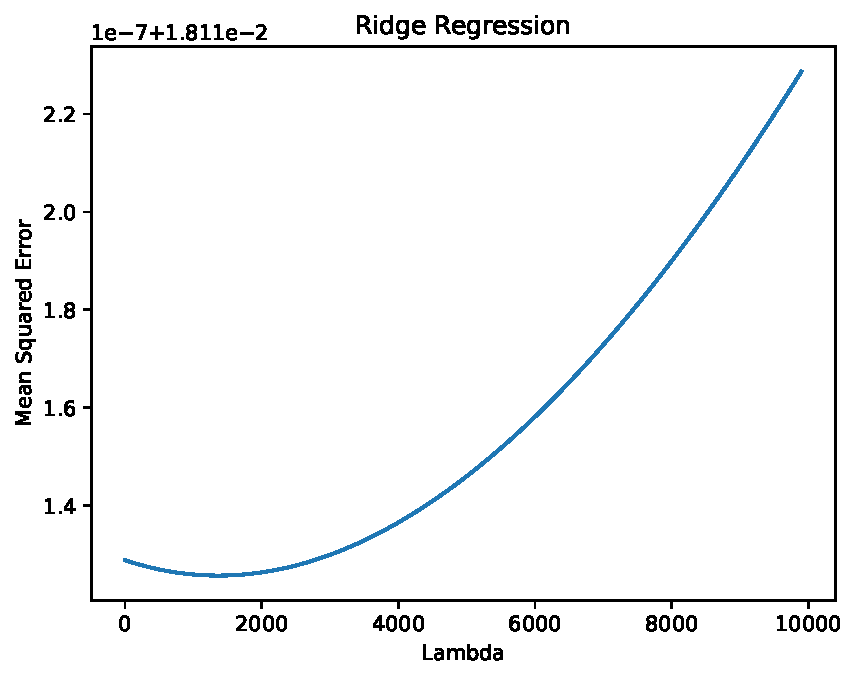
\includegraphics[width=.95\textwidth]{out/2_2.pdf}
\end{figure}

\FloatBarrier
\subsection{}
\begin{figure}[htbp]
    \centering
    \caption{The mean squared error on the validation set, as a function of different features.}
    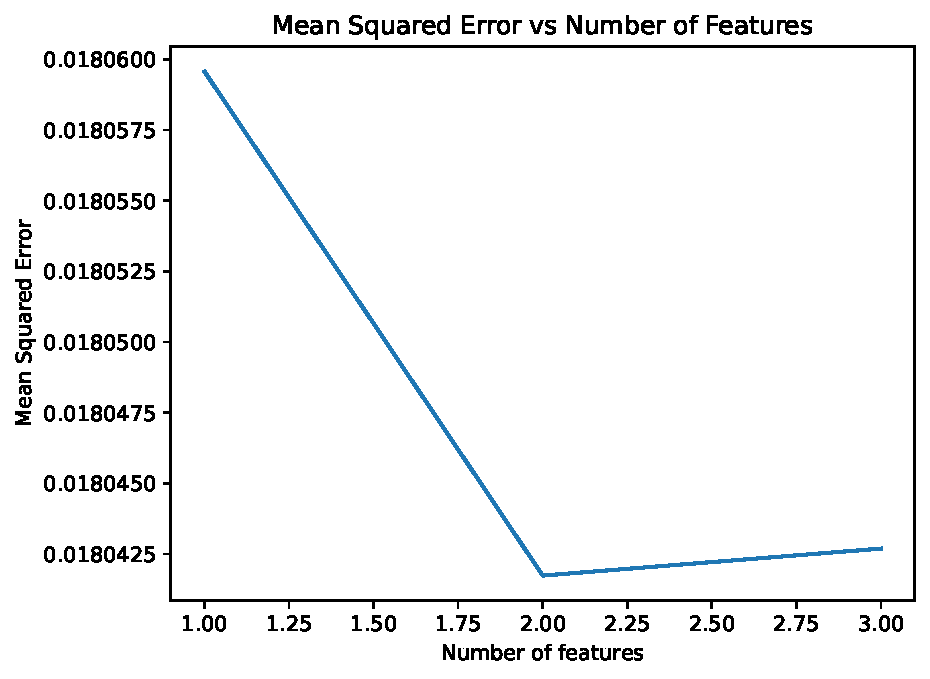
\includegraphics[width=.55\textwidth]{out/2_3_1.pdf}
    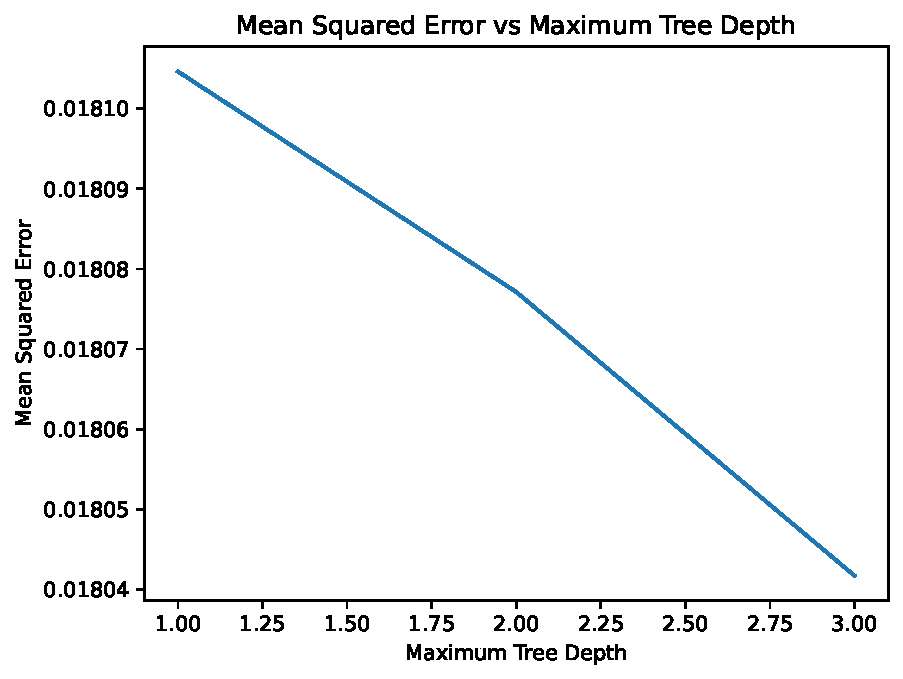
\includegraphics[width=.55\textwidth]{out/2_3_2.pdf}
    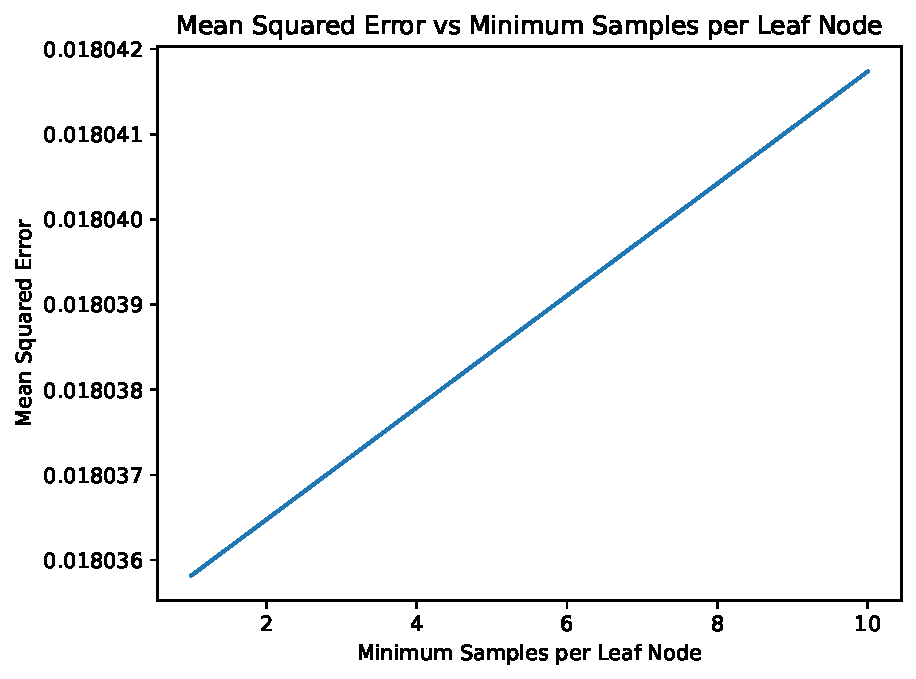
\includegraphics[width=.55\textwidth]{out/2_3_3.pdf}
\end{figure}

\FloatBarrier

% Question 3
\section{}
The results show that both the Pooled OLS (Model A) and Ridge regression (Model B) have the same in-sample R-squared, indicating that they explain a similar proportion of the variance in the data. However, the Random Forest model has a higher in-sample R-squared, suggesting that it provides a better fit to the data.

A higher in-sample R-squared indicates that the Random Forest model captures more of the underlying patterns and relationships in the data, leading to a better prediction performance. This could be attributed to the Random Forest's ability to handle non-linear relationships and interactions between variables, which may not be adequately captured by the linear models like Pooled OLS and Ridge regression.

It is important to note that while a higher in-sample R-squared suggests better performance within the training data, it does not necessarily guarantee better out-of-sample prediction accuracy. Therefore, it is crucial to evaluate the models' performance on unseen data to assess their generalization ability.
\begin{table}[htbp]
    \centering
    \caption{The In-sample R-squared for the Pooled OLS, Ridge Regression, and Random Forest.}
    \resizebox{!}{!}{\begin{tabular}{cc}
\hline
  Model  &  In-sample R2  \\
\hline
 Model A &     0.0012     \\
 Model B &     0.0010     \\
 Model C &     0.0010     \\
\hline
\end{tabular}}
\end{table}
\FloatBarrier

% Question 4
\section{}
In this analysis, we explore the feature importance of each model: Pooled OLS, Ridge regression, and Random Forest. While both Pooled OLS and Ridge regression assign equal importance to the features, they both highlight the significance of the lagged return as the most influential factor. This aligns with existing literature, which suggests that the 12-month momentum serves as a robust predictor of future returns.
However, where the models diverge is in the importance they assign to other features. 
\begin{figure}[htbp]
    \centering
    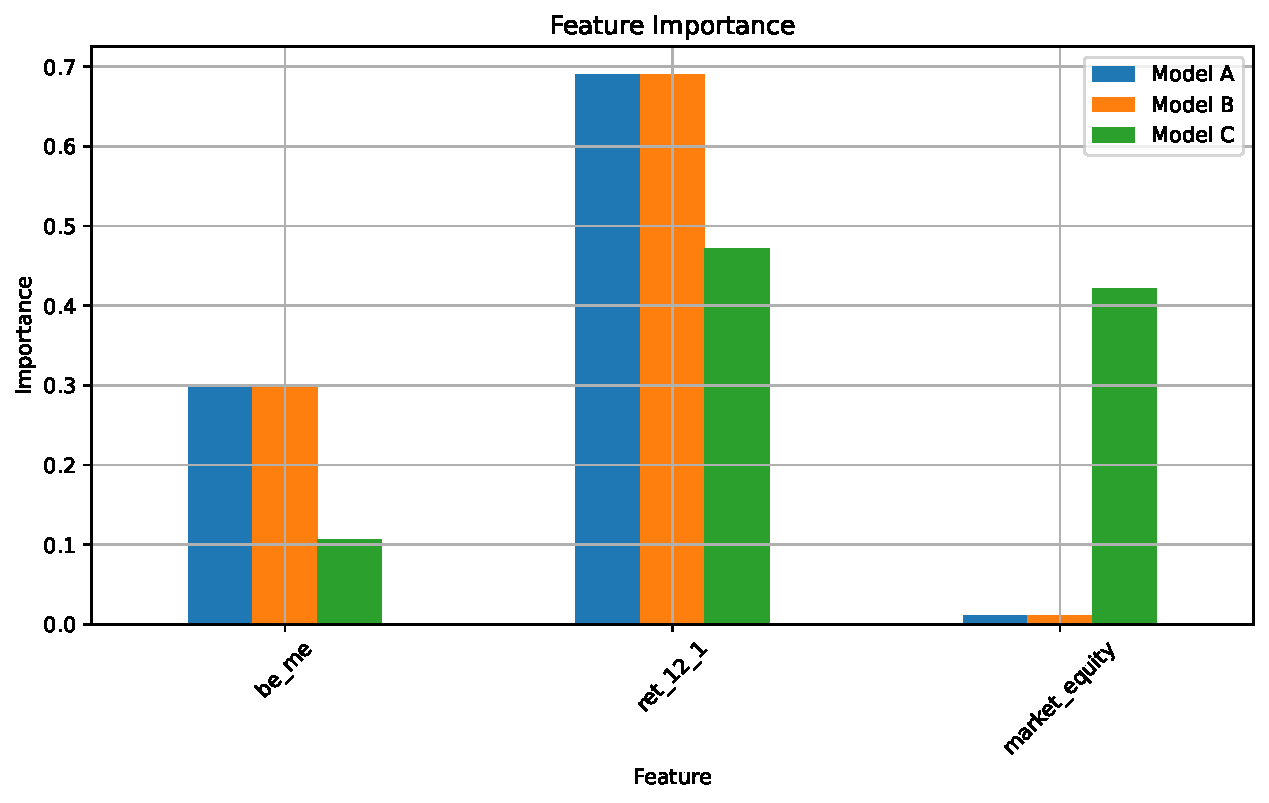
\includegraphics[width=.75\textwidth]{out/4.pdf}
\end{figure}
\FloatBarrier

% Question 5
\section{}

\subsection{}
Here we compare the out-of-sample performance of the Pooled OLS, Ridge regression, and Random Forest models. The results show that the Pooled OLS outperform the Ridge regression and Random Forest in terms of out-of-sample R-squared. This suggests that the Pooled OLS model provides a better fit to the data and captures more of the underlying patterns and relationships, leading to better prediction performance. 
\begin{table}[htbp]
    \centering
    \caption{Out-of-sample R-squared for the Pooled OLS, Ridge Regression, and Random Forest.}
    \resizebox{!}{!}{\begin{tabular}{cc}
\hline
  Model  &  Out-sample R2  \\
\hline
 Model A &     0.2471      \\
 Model B &     0.0010      \\
 Model C &     0.0010      \\
\hline
\end{tabular}}
\end{table}
\FloatBarrier
\subsection{}
I followed the instruction and create 5 portfolios based on the predicted returns for each model. The results show that the Ridge regression outperforms the Pooled OLS and Random Forest in terms of the Sharpe ratio. This suggests that the Ridge regression model provides a better risk-adjusted return, which is an important measure of investment performance.
\begin{table}[htbp]
    \centering
    \caption{Portfolio performance based on the predicted returns for the Pooled OLS, Ridge Regression, and Random Forest.}
    \caption*{\scriptsize\textmd{Panel A: Pooled OLS}}
    \resizebox{0.65\textwidth}{!}{\begin{tabular}{ccccccc}
\toprule
Portfolio & $r_i - r_f$ & $t_{stat}$ & $\alpha_{CAPM}$ & $t_{\alpha}$ & Sharpe Ratio & IR \\
\midrule
1 & 0.008 & 1.621 & 0.008 & 1.472 & 0.149 & 0.139 \\
2 & 0.008 & 1.551 & 0.008 & 1.447 & 0.142 & 0.134 \\
3 & 0.006 & 1.160 & 0.006 & 1.146 & 0.106 & 0.105 \\
4 & 0.009 & 1.798 & 0.009 & 1.767 & 0.165 & 0.162 \\
5 & 0.003 & 0.825 & 0.003 & 0.938 & 0.076 & 0.082 \\
LS & -0.005 & -1.515 & -0.004 & -1.200 & -0.139 & -0.118 \\
\bottomrule
\end{tabular}
}
    
    \vspace{0.5cm} % Add space between tables
    
    \caption*{\scriptsize\textmd{Panel B: Ridge Regression}}
    \resizebox{0.65\textwidth}{!}{\begin{tabular}{ccccccc}
\toprule
Portfolio & $r_i - r_f$ & $t_{stat}$ & $\alpha_{CAPM}$ & $t_{\alpha}$ & Sharpe Ratio & IR \\
\midrule
1 & -0.481 & -0.787 & -0.526 & -0.816 & -0.072 & -0.079 \\
2 & 0.061 & 0.802 & 0.075 & 0.885 & 0.074 & 0.092 \\
3 & -0.010 & -0.168 & -0.012 & -0.226 & -0.015 & -0.019 \\
4 & 0.003 & 0.071 & 0.003 & 0.080 & 0.007 & 0.006 \\
5 & 0.060 & 1.770 & 0.055 & 1.848 & 0.162 & 0.149 \\
LS & 0.540 & 0.884 & 0.580 & 0.900 & 0.081 & 0.087 \\
\bottomrule
\end{tabular}
}
    
    \vspace{0.5cm} % Add space between tables
    
    \caption*{\scriptsize\textmd{Panel C: Random Forest}}
    \resizebox{0.65\textwidth}{!}{\begin{tabular}{ccccccc}
\toprule
Portfolio & $r_i - r_f$ & $t_{stat}$ & $\alpha_{CAPM}$ & $t_{\alpha}$ & Sharpe Ratio & IR \\
\midrule
1 & -0.068 & -0.380 & -0.074 & -0.413 & -0.035 & -0.038 \\
2 & -0.019 & -1.221 & -0.020 & -1.214 & -0.112 & -0.120 \\
3 & -0.059 & -0.745 & -0.032 & -0.510 & -0.068 & -0.038 \\
4 & 0.008 & 1.676 & 0.008 & 1.605 & 0.154 & 0.147 \\
5 & 0.013 & 2.508 & 0.012 & 2.334 & 0.230 & 0.222 \\
LS & 0.080 & 0.452 & 0.086 & 0.485 & 0.041 & 0.045 \\
\bottomrule
\end{tabular}
}
\end{table}
\FloatBarrier

\section{}
Now I use all the mentioned features to predict the returns. Unfortunately, my results for the Random forest model do not look reasonable and I could not fix the problem. I presented the results here following the previous structure. But I cannot discuss these results as they are not reliable.
\renewcommand{\thesubsection}{\thesection.\arabic{subsection}}
\renewcommand{\thesubsubsection}{\thesubsection.\alph{subsubsection}}
\setcounter{subsection}{1}
\subsection{}
\subsubsection{}
\begin{table}[htbp]
    \centering
    \caption{The results of the Pooled OLS regression.}
    \resizebox{.9\textwidth}{!}{\begin{tabular}{lcccccc}
\toprule
                        & \textbf{Parameter} & \textbf{Std. Err.} & \textbf{T-stat} & \textbf{P-value} & \textbf{Lower CI} & \textbf{Upper CI}  \\
\midrule
\textbf{be\_me}         &       0.0041       &       0.0128       &      0.3203     &      0.7487      &      -0.0210      &       0.0292       \\
\textbf{ret\_12\_1}     &       0.0042       &       0.0048       &      0.8691     &      0.3848      &      -0.0053      &       0.0137       \\
\textbf{market\_equity} &       0.1608       &       0.1310       &      1.2274     &      0.2197      &      -0.0959      &       0.4175       \\
\textbf{ret\_1\_0}      &       0.0012       &       0.0048       &      0.2500     &      0.8026      &      -0.0081      &       0.0105       \\
\textbf{rvol\_252d}     &       0.0001       &       0.0109       &      0.0116     &      0.9907      &      -0.0213      &       0.0215       \\
\textbf{beta\_252d}     &      -0.0947       &       0.0857       &     -1.1057     &      0.2688      &      -0.2627      &       0.0732       \\
\textbf{qmj\_safety}    &       0.0068       &       0.0035       &      1.9140     &      0.0556      &      -0.0002      &       0.0137       \\
\textbf{rmax1\_21d}     &      -0.0931       &       0.1244       &     -0.7484     &      0.4542      &      -0.3370      &       0.1507       \\
\textbf{chcsho\_12m}    &      -0.0089       &       0.0621       &     -0.1438     &      0.8856      &      -0.1307      &       0.1129       \\
\textbf{ni\_me}         &      -0.0562       &       0.0472       &     -1.1901     &      0.2340      &      -0.1486      &       0.0363       \\
\textbf{eq\_dur}        &       43.781       &       43.188       &      1.0137     &      0.3107      &      -40.865      &       128.43       \\
\textbf{ret\_60\_12}    &      -0.0098       &       0.0042       &     -2.3206     &      0.0203      &      -0.0180      &      -0.0015       \\
\textbf{ope\_be}        &      -0.0192       &       0.0309       &     -0.6206     &      0.5349      &      -0.0798      &       0.0414       \\
\textbf{gp\_at}         &       0.0024       &       0.0029       &      0.8322     &      0.4053      &      -0.0033      &       0.0081       \\
\textbf{ebit\_sale}     &      -0.6719       &       0.6837       &     -0.9827     &      0.3258      &      -2.0119      &       0.6682       \\
\textbf{at\_gr1}        &      -1.0733       &       0.7334       &     -1.4635     &      0.1433      &      -2.5107      &       0.3641       \\
\textbf{sale\_gr1}      &       0.2397       &       0.2739       &      0.8753     &      0.3814      &      -0.2971      &       0.7765       \\
\textbf{at\_be}         &       0.0777       &       0.0427       &      1.8208     &      0.0686      &      -0.0059      &       0.1613       \\
\textbf{cash\_at}       &      -0.0002       &       0.0030       &     -0.0562     &      0.9552      &      -0.0060      &       0.0057       \\
\textbf{age}            &       9.9438       &       7.5646       &      1.3145     &      0.1887      &      -4.8827      &       24.770       \\
\textbf{z\_score}       &       0.0423       &       0.0594       &      0.7122     &      0.4764      &      -0.0741      &       0.1588       \\
\bottomrule
\end{tabular}
%\caption{Parameter Estimates}}
\end{table}
\FloatBarrier
\subsubsection{}
\begin{figure}[htbp]
    \centering
    \caption{The mean squared error on the validation set, as a function of $\lambda$.}
    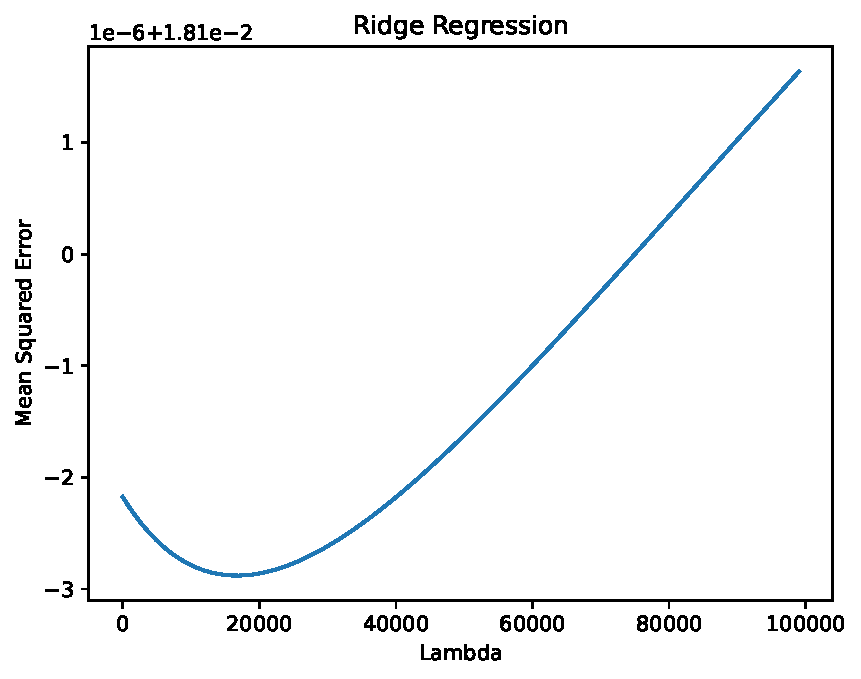
\includegraphics[width=.95\textwidth]{out/6_2.pdf}
\end{figure}
\FloatBarrier
\subsubsection{}
\begin{figure}[htbp]
    \centering
    \caption{The mean squared error on the validation set, as a function of different features.}
    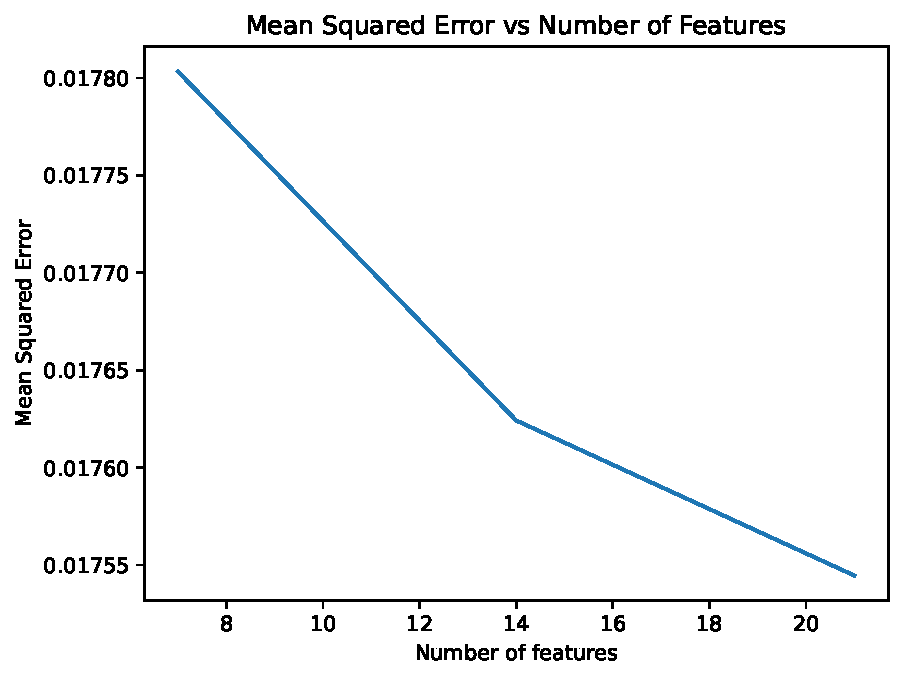
\includegraphics[width=.75\textwidth]{out/6_3_1.pdf}
    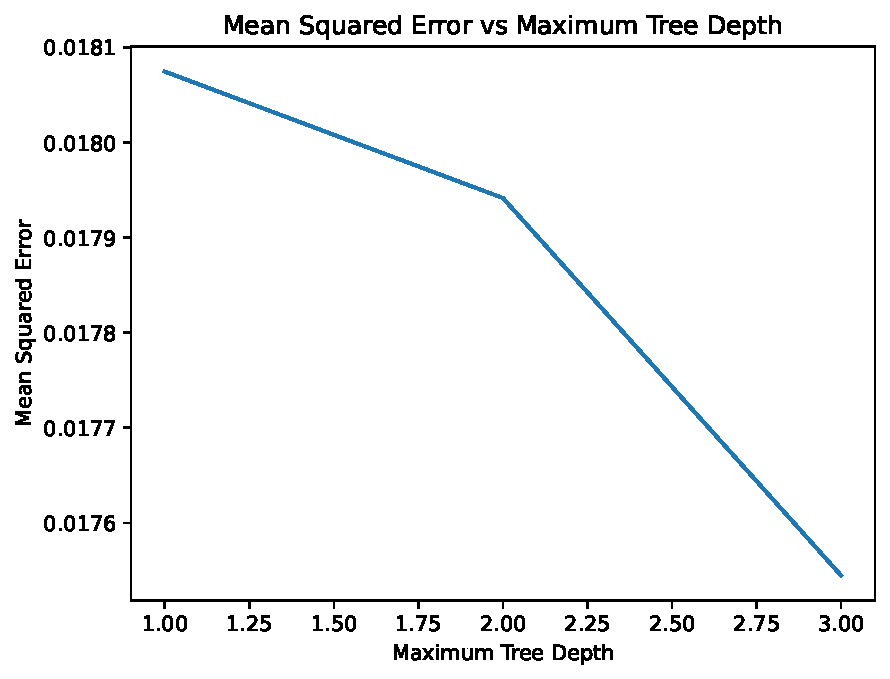
\includegraphics[width=.75\textwidth]{out/6_3_2.pdf}
    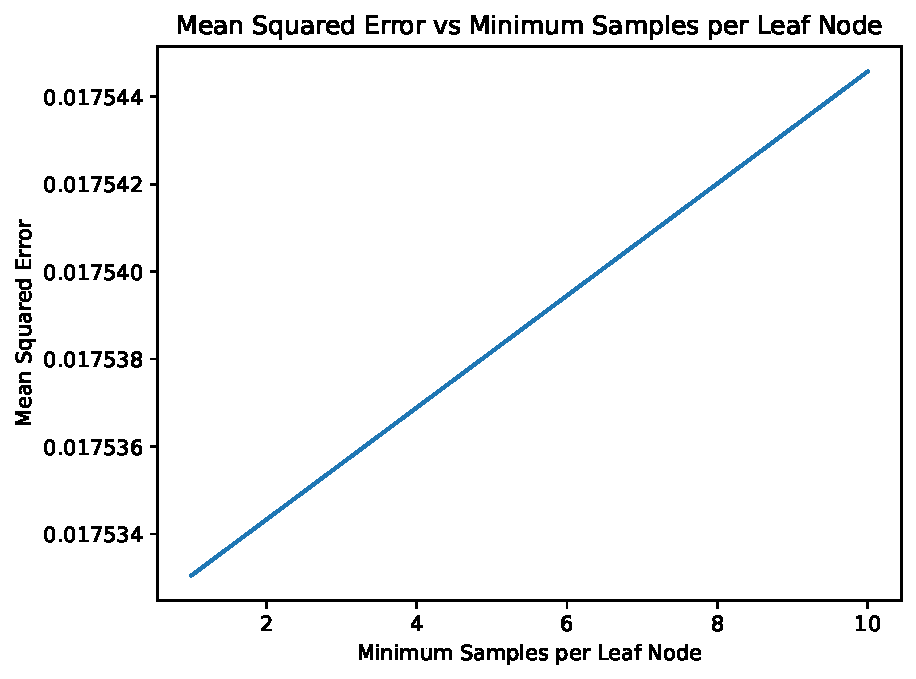
\includegraphics[width=.75\textwidth]{out/6_3_3.pdf}
\end{figure}

\subsection{}
\begin{table}[htbp]
    \centering
    \caption{The In-sample R-squared for the Pooled OLS, Ridge Regression, and Random Forest.}
    \resizebox{!}{!}{\begin{tabular}{cc}
\hline
  Model  &  In-sample R2  \\
\hline
 Model A &     0.0023     \\
 Model B &     0.0023     \\
 Model C &     0.0324     \\
\hline
\end{tabular}}
\end{table}

\FloatBarrier
\section{}

\begin{figure}[htbp]
    \centering
    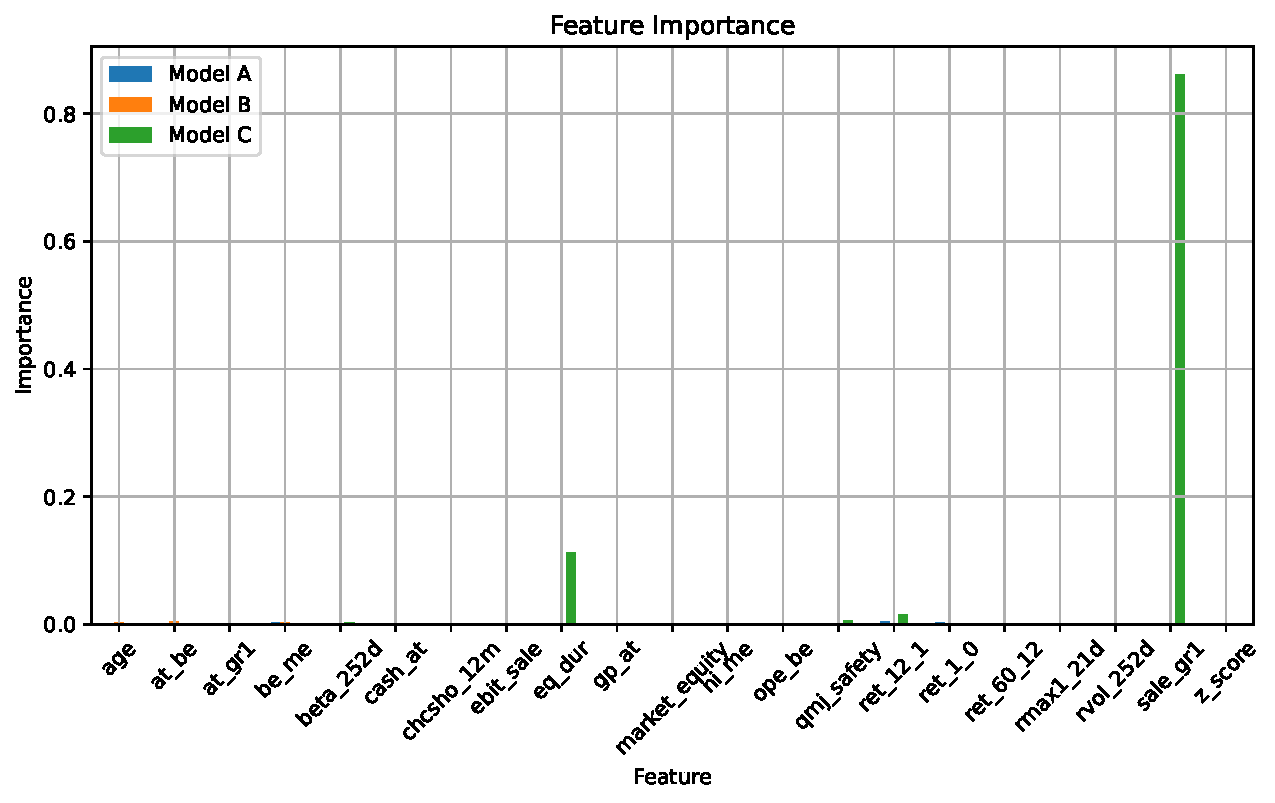
\includegraphics[width=.75\textwidth]{out/6_4.pdf}
\end{figure}
\FloatBarrier
\section{}
\subsection{}
\begin{table}[htbp]
    \centering
    \caption{Out-of-sample R-squared for the Pooled OLS, Ridge Regression, and Random Forest.}
    \resizebox{!}{!}{\begin{tabular}{cc}
\hline
  Model  &  Out-sample R2  \\
\hline
 Model A &     0.4870      \\
 Model B &     0.0002      \\
 Model C &     -0.0298     \\
\hline
\end{tabular}}
\end{table}
\FloatBarrier
\subsection{}
\begin{table}[htbp]
    \centering
    \caption{Portfolio performance based on the predicted returns for the Pooled OLS, Ridge Regression, and Random Forest.}
    \caption*{\scriptsize\textmd{Panel A: Pooled OLS}}
    \resizebox{0.65\textwidth}{!}{\begin{tabular}{ccccccc}
\toprule
Portfolio & $r_i - r_f$ & $t_{stat}$ & $\alpha_{CAPM}$ & $t_{\alpha}$ & Sharpe Ratio & IR \\
\midrule
1 & -0.063 & -1.113 & -0.069 & -1.131 & -0.102 & -0.112 \\
2 & -0.005 & -0.233 & 0.008 & 0.329 & -0.021 & 0.034 \\
3 & 0.091 & 1.510 & 0.084 & 1.545 & 0.138 & 0.129 \\
4 & 0.058 & 1.653 & 0.057 & 1.888 & 0.152 & 0.149 \\
5 & -0.055 & -1.165 & -0.059 & -1.248 & -0.107 & -0.114 \\
LS & 0.008 & 0.111 & 0.011 & 0.127 & 0.010 & 0.013 \\
\bottomrule
\end{tabular}
}
    
    \vspace{0.5cm} % Add space between tables
    
    \caption*{\scriptsize\textmd{Panel B: Ridge Regression}}
    \resizebox{0.65\textwidth}{!}{\begin{tabular}{ccccccc}
\toprule
Portfolio & $r_i - r_f$ & $t_{stat}$ & $\alpha_{CAPM}$ & $t_{\alpha}$ & Sharpe Ratio & IR \\
\midrule
1 & 0.036 & 1.191 & 0.034 & 1.006 & 0.109 & 0.105 \\
2 & -0.004 & -0.410 & -0.003 & -0.343 & -0.038 & -0.030 \\
3 & -0.451 & -1.044 & -0.659 & -1.299 & -0.096 & -0.152 \\
4 & 0.018 & 1.448 & 0.017 & 1.126 & 0.133 & 0.120 \\
5 & 0.017 & 3.061 & 0.017 & 2.804 & 0.281 & 0.271 \\
LS & -0.018 & -0.619 & -0.018 & -0.536 & -0.057 & -0.055 \\
\bottomrule
\end{tabular}
}
    
    \vspace{0.5cm} % Add space between tables
    
    \caption*{\scriptsize\textmd{Panel C: Random Forest}}
    \resizebox{0.65\textwidth}{!}{\begin{tabular}{ccccccc}
\toprule
Portfolio & $r_i - r_f$ & $t_{stat}$ & $\alpha_{CAPM}$ & $t_{\alpha}$ & Sharpe Ratio & IR \\
\midrule
1 & -0.061 & -0.995 & -0.032 & -286097475885977.312 & -0.091 & -3264846760324056.000 \\
2 & 0.402 & 0.785 & 0.142 & 2248224154820543.750 & 0.072 & 7224655780888126.000 \\
3 & 0.115 & 1.281 & -15.369 & -1691176820516556.250 & 0.117 & -10169850206690330.000 \\
4 & 0.061 & 7.593 & 0.151 & 559173050015646.000 & 0.696 & 6160577553020680.000 \\
5 & -0.073 & -34.301 & 0.018 & 275850033277120.750 & -3.144 & 3695901578164656.500 \\
LS & -0.034 & -17.384 & 0.050 & 1224457471030904.000 & -1.594 & 5112797549406387.000 \\
\bottomrule
\end{tabular}
}
\end{table}
\FloatBarrier


\FloatBarrier
\appendix

\section*{Appendix}

Here you can find the python code that I used to solve the exercise. \href{https://github.com/mortezaaghajanzadeh/BDAP/tree/main/Assignments/Assignment 4}{Link to the GitHub repository.}

\end{document}